%---------- Inleiding ---------------------------------------------------------

% TODO: Is dit voorstel gebaseerd op een paper van Research Methods die je
% vorig jaar hebt ingediend? Heb je daarbij eventueel samengewerkt met een
% andere student?
% Zo ja, haal dan de tekst hieronder uit commentaar en pas aan.

%\paragraph{Opmerking}

% Dit voorstel is gebaseerd op het onderzoeksvoorstel dat werd geschreven in het
% kader van het vak Research Methods dat ik (vorig/dit) academiejaar heb
% uitgewerkt (met medesturent VOORNAAM NAAM als mede-auteur).
% 

\section{Inleiding}%
\label{sec:inleiding}

In dit onderzoek wordt een klantomgeving voor Evolane ontwikkeld. 
In deze omgeving worden zowel confidentiële als niet-confidentiële gegevens verwerkt en opgeslagen. 
Door een Data Leakage Prevention-oplossing te implementeren, worden deze gegevens beveiligd tegen lekken. De DLP-oplossing moet ook voldoen aan de Belgische wetgeving, 
waaronder de Algemene Verordening Gegevensbescherming (AVG) over persoonsgegevens (PII) en de Payment Card Industry Data Security Standards (PCI DSS) met betrekking tot betalingsgegevens (PCI). 
De DLP-oplossing moet verder rekening houden met de NIS2-richtlijn en andere cybersecuritykaders, zoals het CCB-kader of ISO 27001. 
De centrale vraag van dit onderzoek is dus: “Hoe kan een op Netskope gebaseerde DLP-oplossing worden ontworpen en geïmplementeerd om vertrouwelijke gegevens te beschermen en te voldoen aan de Belgische regelgeving?”. 
Vanuit deze hoofdvraag kunnen we een aantal deelvragen afleiden:

\begin{itemize}
    \item Welke mogelijkheden biedt Netskope's Secure Service Edge (SSE) platform voor Data Leakage Prevention in de context van vertrouwelijke gegevensbescherming?
    \item Hoe kunnen regelsets en dataclassificatie in Netskope DLP worden afgestemd op de Belgische wetgeving, zoals de AVG en NIS2-richt\-lijn?
    \item Welke technieken en methoden kunnen worden toegepast om persoonsgegevens en betalingsgegevens effectief te detecteren en te beschermen binnen het Net\-skope-platform?
    \item Hoe kan een Proof of Concept (PoC) voor Netskope DLP worden opgezet in een testomgeving om de effectiviteit van de oplossing te evalueren?
    \item Welke juridische en technische normen moeten worden meegenomen bij het ontwerpen van een DLP-oplossing voor een Belgische organisatie, en hoe kan Netskope aan deze eisen voldoen?
\end{itemize}

% Waarover zal je bachelorproef gaan? Introduceer het thema en zorg dat volgende zaken zeker duidelijk aanwezig zijn:

% \begin{itemize}
%   \item kaderen thema
%   \item de doelgroep
%   \item de probleemstelling en (centrale) onderzoeksvraag
%   \item de onderzoeksdoelstelling
% \end{itemize}

% Denk er aan: een typische bachelorproef is \textit{toegepast onderzoek}, wat betekent dat je start vanuit een concrete probleemsituatie in bedrijfscontext, een \textbf{casus}. Het is belangrijk om je onderwerp goed af te bakenen: je gaat voor die \textit{ene specifieke probleemsituatie} op zoek naar een goede oplossing, op basis van de huidige kennis in het vakgebied.
% De doelgroep moet ook concreet en duidelijk zijn, dus geen algemene of vaag gedefinieerde groepen zoals \emph{bedrijven}, \emph{developers}, \emph{Vlamingen}, enz. Je richt je in elk geval op it-professionals, een bachelorproef is geen populariserende tekst. Eén specifiek bedrijf (die te maken hebben met een concrete probleemsituatie) is dus beter dan \emph{bedrijven} in het algemeen.
% Formuleer duidelijk de onderzoeksvraag! De begeleiders lezen nog steeds te veel voorstellen waarin we geen onderzoeksvraag terugvinden.
% Schrijf ook iets over de doelstelling. Wat zie je als het concrete eindresultaat van je onderzoek, naast de uitgeschreven scriptie? Is het een proof-of-concept, een rapport met aanbevelingen, \ldots Met welk eindresultaat kan je je bachelorproef als een succes beschouwen?

%---------- Stand van zaken ---------------------------------------------------

\section{Literatuurstudie}%
\label{sec:literatuurstudie}

\subsection{Data Leakage Prevention (DLP)}%

Een DLP-systeem heeft als doel drie soorten gegevens binnen een organisatie te beschermen: data-at-rest, data-in-motion en data-in-use. 
Data-at-rest verwijst naar statische informatie die is opgeslagen in bedrijfssystemen, zoals documentbeheersystemen, e-mailservers, bestandsservers, netwerkschijven, 
persoonlijke computers en opslagruimtenetwerken (SANs). 
Data-in-motion verwijst naar bedrijfsdata dat wordt verwerkt binnen het uitgaande netwerkverkeer, zoals e-mails en online verkeer. 
Data-in-use bestaat uit informatie die medewerkers gebruiken op eindgebruikersapparaten, zoals een bestand kopiëren naar een USB-schijf. 
De definitie van vertrouwelijkheid binnen een organisatie vereist een grondigere analyse. 
Soorten informatie zoals PII, inclusief namen, identiteitskaart- en creditcardgegevens, worden doorgaans in elke organisatie als vertrouwelijk beschouwd.
Deze definitie krijgt echter ingewikkeldere aspecten bij bedrijfsgeheimen en interne communicatie, die vaak onregelmatig zijn. 
Vertrouwelijke informatie verwijst naar gegevens die binnen de organisatie zijn verzameld en niet algemeen toegankelijk zijn. 
Een DLP-systeem bevat de mogelijkheid om gevoelige gegevens te herkennen in een of meerdere van de genoemde datatypen.

\subsubsection{PCI en PII}

Persoonlijk identificeerbare informatie (PII), zoals namen, rijksregisternummers, e-mail\-adressen, telefoonnummers en dergelijke kunnen direct of indirect worden gebruikt voor de identificatie van een persoon. 
Met het oog op de AVG zijn er strikte regels met betrekking tot toestemming en transparantie bij de verwerking van PII. 
Payment Card Industry (PCI)-gegevens bevatten alle kaart- en betaalgegevens zoals debit-/creditcardnummers, Primary Account Numbers (PAN) en andere confidentiële authenticatiegegevens zoals CVV. 
Om te voldoen aan de PCI DSS-norm (Payment Card Industry Data Security Standard), 
moeten organisaties strenge maatregelen implementeren om deze kaartgegevens te beveiligen. 
Bedrijven die persoonlijk identificeerbare informatie (PII) en PCI-data verwerken lopen het risico op zware sancties als deze gegevens niet voldoende beschermd worden.

\subsubsection{Gegevensverlies detectie methoden}

Identificatiemiddelen worden gebruikt om gevoelige informatie, zoals PII en PCI, te detecteren. 
Dit gebeurt op basis van reguliere expressies (regex). 
Regex is een krachtig hulpmiddel dat DLP helpt specifieke gegevenstypen te herkennen door middel van uitdrukkingen, termen en patronen, 
zoals \texttt{BE\textbackslash d\{2\}\textbackslash s?\textbackslash d\{4\}\textbackslash s?\textbackslash d\{4\}\textbackslash s?\textbackslash d\{4\}} 
dat kan dienen voor Belgische IBAN-codes. Hoewel dit patroon effectief is voor standaard IBAN-formaten, kan het worden omzeild door een karakter toe te voegen in de invoer, 
wat de nood benadrukt van extra controles. 

De aangemaakte identificatie voor confidentiële gegevens moet voldoen aan de volgende richtlijnen:

\begin{itemize}
    \item Vooraf gedefinieerde en aanpasbare patronen voor datadetectie: Het is cruciaal om duizenden vooraf ingestelde regels voor het herkennen van gegevens beschikbaar te hebben en deze te kunnen aanpassen aan de behoeften van de organisatie.
    \item Ondersteuning voor verschillende soorten bestandstypen (Word, Excel, PDF, JPG, PNG, CSV, ZIP en RAR, enz.) en categorieën (afbeeldingen, databases, spreadsheets, enz.).
    \item Ondersteuning voor landspecifieke identificatienummers (IBAN's, postcodes, adressen, nationale identiteitskaarten, IP-adressen, pas\-poort- en telefoonnummers).
    \item Voldoen aan de wet- en regelgeving.
\end{itemize}

De bescherming van PII en PCI-gegevens vormt een kernaspect van DLP. \textcite{Wason2020CASB} legt de nadruk op het belang van de integratie van Cloud Access Security Brokers (CASB) in cloudomgevingen. 
CASB biedt organisaties de mogelijkheid om een uitgebreide zichtbaarheid te krijgen in het gebruik van cloudtoepassingen, inclusief goedgekeurde en ongeautoriseerde (shadow IT) diensten. 
Het houdt bij hoe de confidentiële data wordt opgeslagen en verplaatst/verwerkt, wat handig is voor het identificeren van deze data en het voorkomen van datalekken.

\subsubsection{False Positives}

False positives ontstaan wanneer het DLP-syst\-eem onterecht normale gegevens als confidentieel identificeert. 
Dit kan leiden tot onnodige waarschuwingen en vertragingen in de bedrijfsprocessen. 
Om false positives te vermijden, kan in Netskope bij custom identifiers worden aangegeven dat een bepaald keyword in de buurt moet staan, zoals `RRN' of `Rijksregisternummer'. 
Hierdoor ziet Netskope het niet als een match of zal het een lagere vertrouwheidsscore geven. 

\subsubsection{Detectienauwkeurigheid}

Detectienauwkeurigheid houdt in hoe goed het DLP-systeem in staat is om confidentiële gegevens te identificeren. 
Een hogere detectienauwkeurigheid wordt bereikt door het gebruik van goed afgestemde regelsets en geavanceerde herkenningsmethoden, zoals reguliere expressies (regex), keywords en contextuele analyse.
Netskope maakt gebruik van predefined datasets voor het verbeteren van de detectienauwkeurigheid. 
Deze datasets bevatten gestructureerde gegevens zoals PII en bieden ondersteuning voor verschillende soorten eisen, waaronder de AVG \autocite{Clementelli2023}. 
Netskope maakt ook gebruik van een vertrouwheidsscore om de betrouwbaarheid van de gedetecteerde data te bepalen. 
Deze score helpt bij het evalueren van de waarschijnlijkheid dat bepaalde gegevens confidentieel zijn, 
wat nodig is voor het verminderen van false positives en false negatives. 
Om deze nauwkeurigheid te verhogen, kunnen regelsets aangepast worden aan nieuwe typen confidentiële data of veranderende bedrijfsprocessen.
In deze proof-of-concept wordt de detectienauwkeurigheid beoordeeld door de verhouding tussen true positives, false positives, 
false negatives en true negatives, samengevat in een Confusion Matrix \autocite{Microsoftn.d.}.

\subsubsection{Systeemimpact}

Het meten van de systeemimpact is een belangrijk aspect van DLP-implementaties. 
Indicatoren hierbij zijn CPU-gebruik, geheugengebruik, netwerklatentie, throughput en systeemstabiliteit. 
CPU- en geheugengebruik toont aan hoeveel resources het DLP-systeem op de infrastructuur verbruikt. 
Netwerklatentie en throughput meten de invloed op de netwerkprestaties, 
terwijl systeemstabiliteit aangeeft of het DLP-systeem consistent functioneert zonder storingen. 
Voor het verzamelen en analyseren van deze gegevens kunnen tools zoals \textit{Performance Monitor}, 
\textit{Nagios}, \textit{Zabbix} of de ingebouwde monitoringfunctionaliteiten van Netskope worden ingezet. 

\subsection{Netskope}%

Netskope heeft zich ontwikkeld tot een vooraanstaande speler in cloudbeveiliging door zijn geavanceerde Secure Service Edge (SSE)-platform. 
Het levert geïntegreerde CASB- en DLP-mogelijk\-heden. 
Volgens \textcite{Riley2018} onderscheidt Netskope zich met functies zoals flexibele regelconfiguraties en realtime-detectie van gevoelige data. 
\textcite{VanDerWalt2022} identificeren belangrijke aspecten binnen Secure Access Service Edge (SASE) frameworks die nog onvoldoende onderzoek bevatten. 
Dit combineert netwerk- en beveiligingsdiensten in een cloudgebaseerde omgeving. 
Deze aspecten zijn onder andere de integratie van verschillende beveiligingscomponenten zoals Secure Web Gateways (SWG), CASB en Zero Trust Network Access (ZTNA). 
Deze onderdelen dienen samen te werken om een integrale beveiligingsstrategie te creëren. 
Bovendien is er een toenemende vraag naar het ontwikkelen van API-integraties voor Security Information and Event Management (SIEM)-systemen, 
zodat gegevens uit verschillende bronnen effectief kunnen worden verzameld en geanalyseerd.
% TODO WAAROM NETSKOPE?

Bij het evalueren van DLP-oplossingen binnen een SASE-architectuur is Netskope gekozen vanwege de unieke combinatie van functionaliteiten en prestaties die het biedt, 
evenals de verhouding ten opzichte van andere oplossingen. 
Netskope onderscheidt zich als een volledig geïntegreerd platform binnen het SASE-framework, met een Secure Service Edge (SSE)-oplossing die DLP, CASB, SWG en ZTNA naadloos combineert. 
Deze aanpak is waardevol in gedistribueerde werkomgevingen en bij toenemende cloudadoptie \autocite{brouwer2021cloud}. 
Netskope biedt meer voordelen dan alternatieven zoals Symantec, Digital Guardian, Forcepoint, Microsoft en McAfee. 
Symantec en Digital Guardian richten zich bijvoorbeeld sterk op endpointbeveiliging, maar missen de cloudfunctionaliteiten die nodig zijn in moderne hybride werkomgevingen. 
Forcepoint staat bekend om krachtige gedragsanalyses, maar is minder effectief in het ondersteunen van complexe en dynamische cloudomgevingen. 
Microsoft biedt uitstekende integratie met Office 365, maar hierdoor mist het ook Netskope's cloud-agnostische aanpak, die een breder scala aan cloudapplicaties ondersteunt \autocite{NetskopeTAP2024}. 
Tenslotte biedt McAfee een breed scala aan beveiligingsoplossingen, maar voor Evolane is Netskope een gebruiksvriendelijker platform met meer flexibiliteit bij het opstellen en aanpassen van regelsets.

\subsection{Juridisch kader voor gegevensbescherming in België}%

De bescherming van persoonlijke en bedrijfsinformatie is een essentieel aspect van de hedendaagse digitale samenleving. 
Op zowel nationaal als Europees niveau zijn er wettelijke richtlijnen opgesteld om organisaties te ondersteunen bij het garanderen van de vertrouwelijkheid, 
integriteit en toegankelijkheid van gegevens.

\subsubsection{Algemene Verordening Gegevens\-besch\-erming (AVG)}%

Dit onderzoek zal in overeenstemming zijn met de Algemene Verordening Gegevensbescherming (AVG of GDPR) 2016/679 van 27 april 2016 \autocite{eu_avg2016} en de Belgische wet van 30 juli 2018 \autocite{BelgischeOverheid2018}.
Volgens de \textcite{eu_avg2016}, overweging (78), moeten passende, technische en organisatorische maatregelen worden genomen om de rechten van natuurlijke personen te beschermen. 
Deze overweging zorgt ervoor dat persoonsgegevens op een veilige en verantwoorde manier worden verwerkt. 
Zo'n beveiliging kan gebeuren door middel van standaardinstellingen die erop zijn gericht om risico's in elke fase van de verwerking van gegevens te minimaliseren.
Op 25 juli 2024 publiceerde de Europese Unie haar tweede verslag over de toepassing van de AVG \autocite{eu_avg2024}. 
Dit rapport legt de nadruk op het feit dat de AVG, ondanks verschillende uitdagingen, een goede basis is voor het veilig en transparant behandelen van persoonsgegevens. 


\subsubsection{Payment Card Industry Data Security Standard (PCI DSS)}%

De Payment Card Industry Data Security Stand\-ard (PCI DSS) bestaat uit een reeks richtlijnen en regels die ontworpen zijn voor organisaties die betalingsinformatie en kaartinformatie verwerken, 
zoals debit-/ creditcardnummers, Primary Account Numbers (PAN) en Sensitive Authentication Data (SAD), zoals Card Verification Value (CVV) en magnetische stripgegevens, van alle grote kaartsche\-ma's. 
Deze standaard is ontwikkeld om de veiligheid van kaartinformatie te garanderen en vereist dat organisaties maatregelen nemen om de gegevens van kaarthouders te beschermen \autocite{Elluri2018}. 
PCI DSS vereist de implementatie van toegangscontroles, zoals DCS-02 (toegangscontrole tot systemen en gegevens), DCS-07 (beheer van gebruikersidentiteiten en -toegang), 
en DCS-08 (toegangscontrole tot netwerken en systemen), om de veiligheid van kaartinformatie en de bescherming van kaarthoudergegevens te waarborgen \autocite{Elluri2018}.

\subsubsection{ISO 27001: Informatiebeveiliging}%

Bovendien moet de DLP-oplossing rekening houden met de vereisten van ISO 27001, de internationale norm voor het beheer van informatiebeveiliging. 
In dit verband bespreken \textcite{Alsanabani2020} de noodzaak van DLP-oploss\-ingen die zowel detectie- als preventieve methoden samenbrengen. 
De preventieve aanpak probeert datalekken te vermijden door onder andere het gehele confidentiële bestand te versleutelen, toegangscontrole aan te passen en het labelen van de inhoud.

\subsubsection{Nationale en Europese richtlijnen}%

Buiten de Belgische wetgeving zijn er ook tal van Europese richtlijnen en nationale standaarden die een belangrijke rol hebben in de bescherming van bedrijfsdata. 
Hierbij kan gedacht worden aan de Algemene Verordening Gegevensbescherming (AVG), de EU Cybersecurity Act en belangrijke Europese richtlijnen, waaronder de NIS2-richtlijn. 
Deze richtlijnen worden verder uitgebreid met specifieke normen, zoals de PCI DSS voor betalingsgegevens en internationale normen, zoals ISO 27001 voor de beveiliging van informatie. 
De NIS2-richtlijn (Richtlijn (EU) 2022/2555), die op 16 januari 2023 is aangenomen door de \cite{nis2directive}, 
heeft als doel de cyberbeveiliging binnen de EU te versterken door een hoog niveau van beveiliging te waarborgen voor netwerken en informatiesystemen. 
Artikel 21 van de NIS2-richtlijn richt zich op de beveiliging van netwerken en informatiesystemen en legt de verplichting op aan lidstaten om 
ervoor te zorgen dat aanbieders van essentiële en belangrijke diensten passende technische en organisatorische maatregelen nemen. 
Maatregelen die over het DLP-systeem kunnen gaan, zijn onder andere: 

\begin{itemize}
    \item Risicoanalyse (lid 2, punten a en e): Organisaties moeten een risicobeheerproces implementeren dat hen in staat stelt om risico's voor de beveiliging van netwerken en informatiesystemen te identificeren, te evalueren en te beheersen.
    \item Encryptie en toegangscontroles (lid 2, punten h en i): Het gebruik van encryptie, toegangscontroles en regelmatige beveiligingstests en audits.
    \item Incidentenbehandeling (lid 2, punt b): Organisaties moeten procedures en mechanismen hebben voor het detecteren, melden en reageren op beveiligingsincidenten.
    \item Bewustwording en training (lid 2, punt g): Opleidingen om medewerkers te informeren over goede cyberhygiëne en risicomanagement. \autocite{nis2directive} Het DLP-systeem van Netskope staat in voor het trainen van de eindgebruiker, mocht deze iets foutief doen.
\end{itemize}

De studie van \textcite{Nayak2020} geeft een uitgebreid overzicht van systemen voor het detecteren en voorkomen van datalekken, 
inclusief de indeling van systemen op basis van de status van de gegevens (data-at-rest, data-in-motion, dat\-a-in-use) en de detectietechnieken. 
Dit overzicht zal gebruikt worden voor het ontwikkelen van regex-gebaseerde regels in DLP-oploss\-ingen. 
De studie legt de nadruk op het feit dat datalekken zowel onvoorzien als opzettelijk kunnen optreden en geeft uitdagingen aan, 
zoals het identificeren van gevoelige informatie, het balanceren van de detectienauwkeurigheid en de integratie van geavanceerde methodologieën.

% \subsubsection{Gegevensoverdracht en internationale implicaties}%

\subsubsection{Andere relevante wetgeving}%

De onderstaande tabel bevat de belangrijkste wettelijke richtlijnen en uitspraken die relevant zijn voor het ontwerp en de implementatie van een Data Leakage Prevention-oplossing voor Belgische bedrijven.

\begin{figure}
    \centering
    % \includegraphics[width=.2\textwidth]
    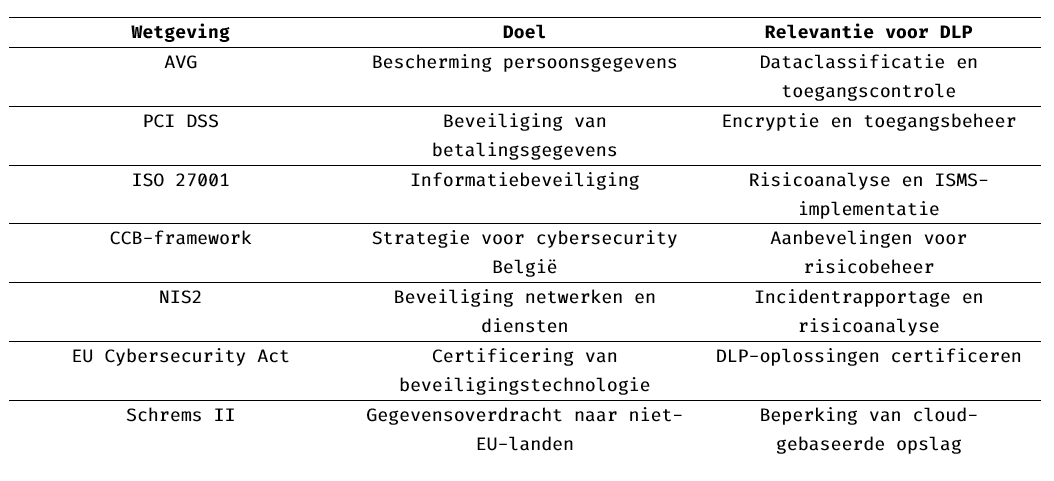
\includegraphics[scale=0.50]
    {img/overzicht.png}
    \caption{\label{fig:overzicht}Overzicht van de belangrijkste wettelijke richtlijnen en uitspraken voor DLP-oplossingen in België.}
  \end{figure}

\subsection{Ethische overwegingen}%

Een essentieel aspect van de implementatie van DLP is het vinden van de juiste balans tussen gegevensbeveiliging en gebruikersprivacy. 
Het gebruik van DLP-systemen kan leiden tot het monitoren van gebruikersgedrag, wat kan worden gezien als een inbreuk op de privacy van medewerkers. 
Om het vertrouwen bij medewerkers en klanten te behouden, is het belangrijk om transparant te zijn over het gebruik van DLP-systemen en de redenen daarvoor. 
Hierdoor weet elke gebruiker welke gegevens worden verzameld en hoe deze worden gebruikt \autocite{Zaini2024}. 
Deze regelsets moeten niet alleen voldoen aan de wettelijke vereisten, maar ook aan de ethische normen en waarden van de organisatie. 
Om monitoring van data en gebruikersgedrag te minimaliseren, 
zal de implementatie van de DLP-oplossing specifiek gericht zijn op het beschermen van gevoelige gegevens en het voorkomen van datalekken. 

% Hier beschrijf je de \emph{state-of-the-art} rondom je gekozen onderzoeksdomein, d.w.z.\ een inleidende, doorlopende tekst over het onderzoeksdomein van je bachelorproef. Je steunt daarbij heel sterk op de professionele \emph{vakliteratuur}, en niet zozeer op populariserende teksten voor een breed publiek. Wat is de huidige stand van zaken in dit domein, en wat zijn nog eventuele open vragen (die misschien de aanleiding waren tot je onderzoeksvraag!)?

% Je mag de titel van deze sectie ook aanpassen (literatuurstudie, stand van zaken, enz.). Zijn er al gelijkwaardige onderzoeken gevoerd? Wat concluderen ze? Wat is het verschil met jouw onderzoek?

% Verwijs bij elke introductie van een term of bewering over het domein naar de vakliteratuur, bijvoorbeeld~\autocite{Hykes2013}! Denk zeker goed na welke werken je refereert en waarom.

% Draag zorg voor correcte literatuurverwijzingen! Een bronvermelding hoort thuis \emph{binnen} de zin waar je je op die bron baseert, dus niet er buiten! Maak meteen een verwijzing als je gebruik maakt van een bron. Doe dit dus \emph{niet} aan het einde van een lange paragraaf. Baseer nooit teveel aansluitende tekst op eenzelfde bron.

% Als je informatie over bronnen verzamelt in JabRef, zorg er dan voor dat alle nodige info aanwezig is om de bron terug te vinden (zoals uitvoerig besproken in de lessen Research Methods).

% % Voor literatuurverwijzingen zijn er twee belangrijke commando's:
% % \autocite{KEY} => (Auteur, jaartal) Gebruik dit als de naam van de auteur
% %   geen onderdeel is van de zin.
% % \textcite{KEY} => Auteur (jaartal)  Gebruik dit als de auteursnaam wel een
% %   functie heeft in de zin (bv. ``Uit onderzoek door Doll & Hill (1954) bleek
% %   ...'')

% Je mag deze sectie nog verder onderverdelen in subsecties als dit de structuur van de tekst kan verduidelijken.

%---------- Methodologie ------------------------------------------------------
\section{Methodologie}%
\label{sec:methodologie}

Het onderzoek naar de ontwikkeling en integratie van een Netskope-gebaseerde Data Leakage Prevention (DLP)-oplossing binnen 
de bedrijfsomgeving van Evolane. De onderzoeksmethode is een combinatie van een uitgebreide literatuurstudie en een praktische Proof of Concept (PoC).

% Feedback op literatuurstudie:
% Het voorstel biedt een sterke basis voor onderzoek met zowel academische als praktische waarde. De combinatie van juridische en technische aspecten maakt het bijzonder relevant voor organisaties die te maken hebben met uitdagingen rond dataveiligheid en compliance. Om het voorstel te versterken, is meer aandacht nodig voor risicoanalyse, gebruikersbetrokkenheid en meetbare criteria alsook de methodologie moet nog verder ontwikkeld worden. Het voorstel is daarom ontvankelijk onder voorwaarden.

% De focus op Belgische regelgeving, zoals de AVG, de NIS2-richtlijn en PCI DSS, geeft het onderzoek een solide juridische onderbouwing en praktische relevantie. De keuze voor Evolane als concrete casus is een duidelijke meerwaarde. Hoewel Netskope een logische keuze lijkt, kan een korte evaluatie van alternatieve DLP-oplossingen of een verduidelijking van de keuze voor Netskope de argumentatie versterken.

% Het voorstel is helder gestructureerd, met een duidelijke hoofdvraag en goed afgebakende deelvragen. De resultaten zullen niet alleen waardevol zijn voor organisaties die Netskope willen implementeren, maar kunnen ook dienen als referentiepunt voor vergelijkbare DLP-oplossingen. Wel ontbreekt er aandacht voor de uitdagingen bij implementatie, zoals het aanpassen van regelsets aan de Belgische regelgeving of het trainen van eindgebruikers.

% Verder mist het voorstel een analyse van potentiële risico’s, zoals technische beperkingen, dataclassificatiefouten of juridische complicaties bij onjuiste configuratie. Ook is er een gebrek aan specificiteit in het meten van de effectiviteit van de Proof of Concept. KPI’s zoals detectienauwkeurigheid, false positives en systeemimpact kunnen hier worden opgenomen. Daarnaast is een bespreking van ethische aspecten, zoals de balans tussen beveiliging en gebruikersprivacy, essentieel.

% Het methodologische luik is onderontwikkeld. Er is geen duidelijke indicatie van de benodigde tijd, middelen of expertise om het onderzoek uit te voeren. Door dit verder uit te werken, kan het voorstel vollediger en realistischer worden gemaakt.

\subsection{Literatuurstudie}%

Het onderzoek begint met een uitgebreide literatuurstudie naar bestaande DLP-oplossingen, Netskope's Secure Service Edge (SSE) platform en de relevante Belgische en Europese wetgeving. 
Hierbij wordt gebruikgemaakt van academische artikelen, technische documentatie en juridische bronnen om een basis te leggen. 
Voor de literatuurstudie is ongeveer twee weken voorzien, waarin de focus ligt op het verder verzamelen en verwerken van recente bronnen
over DLP-technologie, juridische eisen (AVG, PCI DSS, NIS2) en Netskope's DLP-oplossing.

\subsection{Analyse en planning}%

Na de literatuurstudie worden specifieke datasetsspecifieke datasets, zoals persoonlijk identificeerbare informatie (PII) 
en betalingsgegevens (PCI), geselecteerd voor testen binnen de PoC. 
bijvoorbeeld de synthetische e-maildatasets van \textcite{Whelan2014}.
Deze datasets bevatten in totaal 4796 e-mails, waarvan 4010 geen PII bevatten en 786 e-mails dit wel hebben, 
waaronder adressen, creditcardnummers en namen. 
Ook worden realistische testscenario's opgesteld die aansluiten bij de bedrijfsprocessen van Evolane, zoals e-mailverkeer en bestandsoverdrachten 
naar cloudservices. Een projectplan zal hier ook uitgewerkt worden, waarin de benodigde middelen, zoals Netskope-licenties en testservers, worden 
geïdentificeerd. Verder zal hierin ook de tijdsplanning, inclusief de deliverables, worden opgenomen.
Deze fase begint al deels tijdens de literatuurstudie en duurt ongeveer drie weken.

\subsection{Risicoanalyse}%

Een belangrijk onderdeel van dit onderzoek is het uitvoeren van een risicoanalyse, waarbij mogelijke technische, juridische en organisatorische risico's worden geïdentificeerd en beoordeeld.
Technische risico's kunnen bijvoorbeeld bestaan uit het niet volledig detecteren van gevoelige gegevens of prestatieproblemen van het DLP-systeem. 
Juridische risico's hebben te maken met het niet naleven van de AVG-vereisten of andere relevante wetgeving. 
Organisatorische risico's omvatten mogelijke weerstand van medewerkers tegen nie\-uwe beveiligingsmaatregelen of een gebrek aan training, 
wat de effectiviteit van de DLP-oplossing kan verminderen.
Voor elk vastgesteld risico worden geschikte maatregelen genomen om de gevolgen te beperken.
Deze fase duurt ongeveer twee weken, overlappend met Analyse en Planning. Op het vlak van expertise zal hierbij de co-promotor van Evolane betrokken worden.

\subsubsection{Technische risico's}

Technische risico's zijn gerelateerd aan de operationele elementen van de DLP-oplossing en de technische infrastructuur van Evolane.
Een van de belangrijkste technische risico's is de onvolledige detectie van confidentiële gegevens. 
Het DLP-systeem kan mogelijk niet alle vormen van PII en PCI detecteren, vooral als er nieuwe of onbekende datatypes worden gebruikt.
Daarnaast kan de implementatie van Netskope leiden tot prestatieproblemen, zoals vertragingen in netwerkverkeer of een verhoogd gebruik van systeemresources.
Integratieproblemen vormen een ander potentieel risico, aangezien het DLP-systeem moet werken met bestaande IT-infrastructuren.
Onverwachte compatibiliteitsproblemen kunnen de implementatie vertragen. Vervolgens kunnen verdere beveiligingslekken ontstaan 
door onvoldoende configuratie of zwakke punten in het DLP-systeem, waardoor confidentiële data alsnog kan worden gelekt.
Om deze technische risico's te mitigeren, zullen uitgebreide tests worden uitgevoerd om de detectienauwkeurigheid van het DLP-systeem te waarborgen.
Daarnaast zullen systeemprestaties worden gemonitord tijdens de implementatie en indien nodig optimalisaties worden doorgevoerd om prestatieproblemen te minimaliseren.
Tenslotte zal een plan worden opgesteld hoe het DLP-systeem veilig geüpdatet kan worden om potentiële kwetsbaarheden te vermijden.

\subsubsection{Juridische risico's}

Juridische risico's hebben betrekking op de naleving van wet- en regelgeving, zoals de Algemene Verordening Gegevensbescherming (AVG) en de NIS2-richtlijn.
Onvoldoende naleving van deze wetten en richtlijnen (waaronder AVG, PCI DSS, ISO 27001, NIS2, Schrems II,..) kan leiden tot juridische sancties. 
Een belangrijk juridisch risico betreft onjuiste Data Processing Agreements (DPA) met dataverwerkers. 
Verkeerde of ontbrekende overeenkomsten met dataverwerkers kunnen juridische complicaties veroorzaken. 
Daarnaast kan het niet correct toepassen van dataminimalisatieprincipes of het verwerken van data voor andere doeleinden dan waarvoor ze zijn verzameld, 
ook leiden tot juridische gevolgen. 
Om deze juridische risico's te mitigeren, zullen DPA's zorgvuldig worden opgesteld en regelmatig worden herzien met alle betrokken derde partijen. 

\subsubsection{Organisatorische risico's}

Organisatorische risico's hebben betrekking op de interne processen en procedures van Evolane en de acceptatie van de DLP-oplossing door medewerkers. 
Weerstand van medewerkers kan een belangrijk organisatorisch risico vormen, aangezien medewerkers mogelijk niet openstaan voor nieuwe beveiligingsmaatregelen. 
Een gebrek aan training kan bovendien leiden tot misbruik of onjuist gebruik van het DLP-systeem, wat de effectiviteit ervan zal verminderen. 
Om dan tenslotte deze organisatorische risico's te mitigeren, zullen workshops en informatiesessies worden georganiseerd om medewerkers te betrekken en het belang van de DLP-oplossing te benadrukken. 
Door medewerkers actief te betrekken en voldoende training te bieden, wordt het gebruik van de DLP-oplossing vergroot en wordt de effectiviteit ervan versterkt.

\subsection{Proof of Concept}%

De PoC wordt opgezet in een interne testomgeving binnen het bedrijf, waarbij een Netskope-licentie wordt gebruikt om de DLP-service in te stellen. 
Deze omgeving zal verschillende datatypes bevatten (data-in-use, data-in-motion, data-at-rest), 
waarbij zowel vertrouwelijke als niet\--vertr\-ouwelijke bestanden worden gebruikt om te testen of de DLP-service alle vertrouwelijke data effectief kan identificeren en verdere verwerking kan blokkeren. 
De data bestaat voornamelijk uit persoonlijk identificeerbare informatie (PII) en betalingsgegevens (PCI), die volgens de geldende wet- en regelgeving (zoals AVG, PCI DSS, ISO 27001, NIS2, Schrems II, enz.) beschermd moeten worden. 
Gebruikers met verschillende rechten zullen data doorsturen en verwerken binnen de testomgeving. 
De duur van de PoC is afhankelijk van de complexiteit van de testscenario's en de detectie van gevoelige gegevens, 
maar wordt geschat op 5 tot 6 weken. 
Na ongeveer 5 weken zou een eerste evaluatie van de effectiviteit van de DLP-oplossing mogelijk moeten zijn, 
en kan deze aan de eindgebruikers van Evolane worden gepresenteerd. 
Voor de technische uitvoering is expertise nodig in de configuratie van Netskope (bijvoorbeeld het instellen van detectie- en preventieregels met regex-patronen), 
evenals basiskennis van de netwerkinfrastructuur van de testomgeving om de dataflows goed na te bootsen.

\subsection{Gebruikerstests en feedback}%

Na de initiële implementatie van de PoC worden gebruikers van Evolane betrokken bij het testen van de DLP-oplossing. 
Dit gebeurt, samen met mijn co-promotor, door middel van workshops en praktische tests waarbij eindgebruikers realistische scenario's simuleren waarin gevoelige data verwerkt en verplaatst wordt. 
De feedback van deze gebruikers is essentieel om inzicht te krijgen in de gebruiksvriendelijkheid en de invloed van de DLP-regelsets op de dagelijkse taken. 

\subsection{Evaluatie en meetbare criteria}%

De effectiviteit van de geïmplementeerde DLP-oplossing wordt geëvalueerd aan de hand van vooraf gedefinieerde Key Performance Indicators (KPI's). 
Deze KPI's dienen als indicator om te beoordelen in hoeverre de DLP-oplossing voldoet aan de gestelde vereisten en doelstellingen.
Detectienauwkeurigheid meet het percentage correct geïdentificeerde confidentiële gegevens binnen de totale dataset, 
wat aangeeft hoe effectief de DLP-oplossing is in het herkennen van PII en PCI. 
Het aantal false positives geeft aan hoeveel gegevens onterecht zijn geblokkeerd of gemarkeerd, 
wat inzicht geeft in de nauwkeurigheid van de detectiemethoden en helpt bij het finetunen van de regelsets. 
Dit zal in een Confusion Matrix worden weergegeven \autocite{Microsoftn.d.}.
Systeemimpact zal het effect van de DLP-implementatie op de algehele systeemprestaties beoordelen, zoals CPU- en 
geheugenverbruik, zodat de oplossing geen significante vertragingen of resource-uitputting zou veroorzaken.

\subsection{Documentatie van resultaten}%

Alle bevindingen en conclusies worden grondig gedocumenteerd. 
In ongeveer twee weken tijd worden handleidingen, een schriftelijk evaluatierapport en het finale concept-bachelorproef geschreven.

\subsection{Planning}%
\label{sec:planning}

De planning van het onderzoek, weergegeven in Figuur 2, is vastgelegd in een Gantt-diagram. De planning is opgesteld van 17 februari 2025 tot 24 mei 2025, met de laatste twee weken specifiek gereserveerd voor documentatie.

\begin{figure}
    \centering
    % \includegraphics[width=.2\textwidth]
    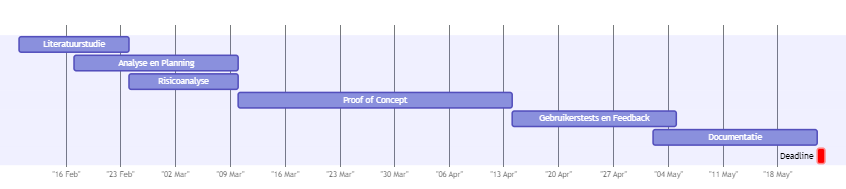
\includegraphics[scale=0.50]
    {img/gantt.png}
    \caption{\label{fig:gant}Gantt-diagram van de onderzoeksplanning van 10 februari 2025 tot 23 mei 2025.}
  \end{figure}

% **Uitleg van het Gantt-diagram**:

% - **Literatuurstudie**: Start op 17 februari en loopt tot 3 maart. Aangezien de literatuurstudie al bijna voltooid is, beslaat deze fase de laatste afrondingen.
% - **Analyse en Planning**: Start op 3 maart en loopt tot 14 maart. In deze fase worden de specifieke datasets geselecteerd en testscenario's opgesteld.
% - **Risicoanalyse**: Start op 14 maart en loopt tot 21 maart. Deze fase omvat het identificeren en evalueren van mogelijke risico's.
% - **Proof of Concept (PoC)**: Start op 21 maart en loopt tot 25 april. Dit is de meest intensieve fase, waarin de testomgeving wordt opgezet, Netskope wordt geconfigureerd, en de PoC wordt uitgevoerd.
% - **Gebruikerstests en Feedback**: Start op 25 april en loopt tot 2 mei. Hierbij worden gebruikers betrokken bij het testen van de DLP-oplossing en wordt feedback verzameld.
% - **Evaluatie en Meetbare Criteria**: Start op 25 april en loopt tot 2 mei. Deze fase omvat de analyse van de testresultaten aan de hand van KPI's.
% - **Documentatie**: Start op 18 april en loopt tot 2 mei. De laatste twee weken zijn gereserveerd voor het documenteren van de resultaten en het afronden van de finale draft.


% Hier beschrijf je hoe je van plan bent het onderzoek te voeren. Welke onderzoekstechniek ga je toepassen om elk van je onderzoeksvragen te beantwoorden? Gebruik je hiervoor literatuurstudie, interviews met belanghebbenden (bv.~voor requirements-analyse), experimenten, simulaties, vergelijkende studie, risico-analyse, PoC, \ldots?

% Valt je onderwerp onder één van de typische soorten bachelorproeven die besproken zijn in de lessen Research Methods (bv.\ vergelijkende studie of risico-analyse)? Zorg er dan ook voor dat we duidelijk de verschillende stappen terug vinden die we verwachten in dit soort onderzoek!

% Vermijd onderzoekstechnieken die geen objectieve, meetbare resultaten kunnen opleveren. Enquêtes, bijvoorbeeld, zijn voor een bachelorproef informatica meestal \textbf{niet geschikt}. De antwoorden zijn eerder meningen dan feiten en in de praktijk blijkt het ook bijzonder moeilijk om voldoende respondenten te vinden. Studenten die een enquête willen voeren, hebben meestal ook geen goede definitie van de populatie, waardoor ook niet kan aangetoond worden dat eventuele resultaten representatief zijn.

% Uit dit onderdeel moet duidelijk naar voor komen dat je bachelorproef ook technisch voldoen\-de diepgang zal bevatten. Het zou niet kloppen als een bachelorproef informatica ook door bv.\ een student marketing zou kunnen uitgevoerd worden.

% Je beschrijft ook al welke tools (hardware, software, diensten, \ldots) je denkt hiervoor te gebruiken of te ontwikkelen.

% Probeer ook een tijdschatting te maken. Hoe lang zal je met elke fase van je onderzoek bezig zijn en wat zijn de concrete \emph{deliverables} in elke fase?

%---------- Verwachte resultaten ----------------------------------------------
\section{Verwacht resultaat, conclusie}%
\label{sec:verwachte_resultaten}

Dit onderzoek zal een volledig uitgewerkt Proof of Concept (PoC) opleveren van een Netskope-gebaseerde DLP-oplossing, die is ontworpen om vertrouwelijke gegevens, 
zoals PII- en PCI-gegeve\-ns, te beschermen volgens de Belgische wetgeving. 
De PoC zal datalekken identificeren en beschermen in een realistische testomgeving die door Evolane mede opgezet zal worden. 
De vertrouwelijke data zullen in alle mogelijke datatypen voorkomen, zoals data-in-use, data-in-motion en data-at-rest. De oplossing zal gericht zijn op 
het voorkomen van datalekken die kunnen optreden bij het verwerken en verplaatsen van gevoelige gegevens, zowel binnen als buiten de organisatie.
De proof-of-concept zal een geconfigureerd DLP-platform opleveren dat PII- en PCI-gege\-vens kan identificeren en beschermen volgens de vooraf ingestelde parameters. 
Deze parameters zullen voldoen aan klant-specifieke dataclassificaties en zullen worden gevalideerd aan de hand van specifieke testscenario's. 
Het resultaat van deze tests wordt gepresenteerd in een evaluatierapport, dat de effectiviteit van de oplossing evalueert.
Daarnaast zal het onderzoek aanbevelingen doen over hoe organisaties de Netskope DLP-oplossing kunnen implementeren om te voldoen aan zowel technische als juridische normen. 
Tijdens de gebruikers- en feedbacktests zullen medewerkers van Evolane betrokken worden bij het testen van de DLP-oplossing en het geven van feedback over de bruikbaarheid en effectiviteit ervan. 
Hierbij zullen hoogstwaarschijnlijk nog enkele aanpassingen aan de regelsets gebeuren om de detectienauwkeurigheid te verbeteren en het aantal false positives te verminderen. 
Het verwacht resultaat omvat een succesvolle implementatie van een DLP-oplossing die effectief de risico's van datalekken vermindert. 

% Hier beschrijf je welke resultaten je verwacht. Als je metingen en simulaties uitvoert, kan je hier al mock-ups maken van de grafieken samen met de verwachte conclusies. Benoem zeker al je assen en de onderdelen van de grafiek die je gaat gebruiken. Dit zorgt ervoor dat je concreet weet welk soort data je moet verzamelen en hoe je die moet meten.

% Wat heeft de doelgroep van je onderzoek aan het resultaat? Op welke manier zorgt jouw bachelorproef voor een meerwaarde?

% Hier beschrijf je wat je verwacht uit je onderzoek, met de motivatie waarom. Het is \textbf{niet} erg indien uit je onderzoek andere resultaten en conclusies vloeien dan dat je hier beschrijft: het is dan juist interessant om te onderzoeken waarom jouw hypothesen niet overeenkomen met de resultaten.
